% =============================================================================
\section{Mean-field approximation}
\label{sec:bec-noise:mean-field}
% =============================================================================

We will start from the classical model of a trapped \abbrev{bec} --- the mean-field approximation.
While it cannot predict quantum effects, it provides the basis for comparison with the truncated Wigner method, and can be also applied to calculate the ground state of a trapped \abbrev{bec} numerically.

We will use the combined model which includes linear coupling and losses, and later in \secref{bec-noise:wigner}, dedicated to the application of the truncated Wigner method we will show how we can get almost identical equations from the first principles.


% =============================================================================
\subsection{Two-component condensate}
% =============================================================================

The classical \abbrev{bec} is described by the wavefunctions $\Psi_j$, which are normalized such that $\int |\Psi_j|^2 \upd\xvec \equiv N_j$, where $N_j$ is the total population of the component $j$ (consequently, $|\Psi_j|^2 \equiv n_j$ is the component density).
The evolution of the condensate is described by the system of coupled Gross-Pitaevskii equations (\abbrev{cgpe}s)
\begin{eqn}
\label{eqn:bec-noise:mean-field:cgpes}
	i \hbar \frac{\upd \Psi_1}{\upd t} ={} & \left(
		-\frac{\hbar^2 \nabla^2}{2 m} + V_1 + \hbar \omega_1^{(i)}
		+ g_{11} \lvert \Psi_1 \rvert^2
		+ g_{12} \lvert \Psi_2 \rvert^2
		- i \hbar \Gamma_1
	\right) \Psi_1 \\
	& + \frac{\hbar \Omega}{2} \left(
		e^{i (\omega t + \alpha)} + e^{-i (\omega t + \alpha)}
	\right) \Psi_2, \\
	i \hbar \frac{\upd \Psi_2}{\upd t} ={} & \left(
		-\frac{\hbar^2 \nabla^2}{2 m} + V_2 + \hbar \omega_2^{(i)}
		+ g_{22} \lvert \Psi_2 \rvert^2
		+ g_{12} \lvert \Psi_1 \rvert^2
		- i \hbar \Gamma_2
	\right) \Psi_2 \\
	& + \frac{\hbar \Omega}{2} \left(
		e^{i (\omega t + \alpha)} + e^{-i (\omega t + \alpha)}
	\right) \Psi_1.
\end{eqn}
Here $V_j(\xvec)$ are external potentials~\eqnref{bec-noise:system:V}, $\omega_j^{(i)}$ is the internal energy of the component $j$, $g_{jk}$ are nonlinear interaction coefficients~\eqnref{bec-noise:system:g}, $\Gamma_j$ terms represent nonlinear losses for the component $j$, and $\Omega$ is the electromagnetic coupling strength (with $\omega$ being the frequency, and $\alpha$ the phase of the coupling).
The \abbrev{cgpe}s without loss or coupling terms were introduced in~\cite{Zeng1995,Ho1996}.
The coupling terms were first included in~\cite{Ballagh1997}, and the loss terms in~\cite{Yurovsky1999}.
A detailed description of the mean-field approximation can be found in~\cite{Pitaevskii2003}.

The exact expression of the loss parameters $\Gamma_j$ depends on the loss processes in the particular experiment.
For example, the dominant three-body and two-body losses in the two-component \Rb{} \abbrev{bec} with the components ${\ket{F=1,\, m_F=-1}}$ and ${\ket{F=2,\, m_F=+1}}$ result in~\cite{Burt1997,Mertes2007}
\begin{eqn}
\label{eqn:bec-noise:mean-field:losses}
	\Gamma_1 &= \left( \gamma_{111} n_1^2 + \gamma_{12} n_2 \right) / 2, \\
	\Gamma_2 &= \left( \gamma_{12} n_1 + \gamma_{22} n_2 \right) / 2.
\end{eqn}
These equations were obtained empyrically, but we will see later in this chapter how the same (in the first-order term) expressions appear as a result of the application of the truncated Wigner method to the exact operator equation.

The difference between the internal energies of spins $1$ and $2$ is the hyperfine frequency $\omega_{hf} = \omega_1^{(i)} - \omega_2^{(i)}$.
The coupling frequency $\omega$ is usually slightly detuned from the hyperfine frequency in the experiment: $\omega = \omega_{hf} + \delta$, where $\delta \ll \omega_{hf}$.

The fact that $\hbar \omega_j \gg V_j$ can cause problems when performing calculations with low precision.
Therefore it is convenient to use equations~\eqnref{bec-noise:mean-field:cgpes} in a rotating frame:
\begin{eqn}
	\Psi_1 & \rightarrow \Psi_1 e^{i \omega_1^{(i)} t}, \\
	\Psi_2 & \rightarrow \Psi_2 e^{i \omega_2^{(i)} t}.
\end{eqn}
This transformation eliminates $\omega_1^{(i)}$ and $\omega_2^{(i)}$ from the equations and does not change single-time observable values.
The transformed equations look like:
\begin{eqn}
	i \hbar \frac{\upd \Psi_1}{\upd t} ={} & \left(
		-\frac{\hbar^2 \nabla^2}{2 m} + V_1
		+ g_{11} \lvert \Psi_1 \rvert^2
		+ g_{12} \lvert \Psi_2 \rvert^2
		- i \hbar \Gamma_1
	\right) \Psi_1 \\
	& + \frac{\hbar \Omega}{2} \left(
		e^{i ((\omega + \omega_{hf}) t + \alpha)} + e^{-i (\delta t + \alpha)}
	\right) \Psi_2, \\
	i \hbar \frac{\upd \Psi_2}{\upd t} ={} & \left(
		-\frac{\hbar^2 \nabla^2}{2 m} + V_2
		+ g_{22} \lvert \Psi_2 \rvert^2
		+ g_{12} \lvert \Psi_1 \rvert^2
		- i \hbar \Gamma_2
	\right) \Psi_2 \\
	& + \frac{\hbar \Omega}{2} \left(
		e^{i (\delta t + \alpha)} + e^{-i ((\omega + \omega_{hf}) t + \alpha)}
	\right) \Psi_1.
\end{eqn}

Furthermore, in the experiment the coupling field is applied for short periods of time $t_{\mathrm{pulse}}$, where $1 / \omega \ll t_{\mathrm{pulse}} \ll 1 / \delta$.
This allows us to neglect the quickly oscillating terms:
\begin{eqn}
\label{eqn:bec-noise:mean-field:cgpes-simplified}
	i \hbar \frac{\upd \Psi_1}{\upd t} & = \left(
		-\frac{\hbar^2 \nabla^2}{2 m} + V_1
		+ g_{11} \lvert \Psi_1 \rvert^2
		+ g_{12} \lvert \Psi_2 \rvert^2
		- i \hbar \Gamma_1
	\right) \Psi_1
	+ \frac{\hbar \Omega}{2} e^{-i (\delta t + \alpha)} \Psi_2, \\
	i \hbar \frac{\upd \Psi_2}{\upd t} & = \left(
		-\frac{\hbar^2 \nabla^2}{2 m} + V_2
		+ g_{22} \lvert \Psi_2 \rvert^2
		+ g_{12} \lvert \Psi_1 \rvert^2
		- i \hbar \Gamma_2
	\right) \Psi_2 +
	\frac{\hbar \Omega}{2} e^{i (\delta t + \alpha)} \Psi_1.
\end{eqn}
When the pulse is applied twice using the same coupling field (which is the case for the Ramsey interferometry), it is the same as just setting $\Omega$ to zero after the first pulse and then restoring its value for the time of the second pulse; therefore $\alpha$ stays the same too.
If one wants to apply pulse with the different detuning, the phase information is lost, and the value of $\alpha$ has to become random before this pulse.

The application of the coupling field can be simplified, if certain additional conditions are valid, namely:
\begin{enumerate}
	\item $\mu / \hbar \ll \Omega$, where $\mu$ is the chemical potential of the first component;
	\item $\delta \ll \Omega$;
	\item the characteristic time of the other terms in~\eqnref{bec-noise:mean-field:cgpes} is much greater than $t_{\mathrm{pulse}}$.
\end{enumerate}
This allows us to use the ``instantaneous'' pulse, multiplying the state vector by a rotation matrix:
\begin{eqn}
\label{eqn:bec-noise:mean-field:rotation-matrix}
	\begin{pmatrix}
		\Psi^\prime_1 \\ \Psi^\prime_2
	\end{pmatrix} =
	\begin{pmatrix}
		\cos \frac{\theta}{2} & -i e^{-i \phi} \sin \frac{\theta}{2} \\
		-i e^{i \phi} \sin \frac{\theta}{2} & \cos \frac{\theta}{2}
	\end{pmatrix}
	\begin{pmatrix}
		\Psi_1 \\ \Psi_2
	\end{pmatrix},
\end{eqn}
where $\theta = \Omega t_{\mathrm{pulse}}$, and $\phi$ is the phase of the coupling field at the beginning of the pulse.
In particular, for the two-pulse Ramsey scheme with the time $t_R$ between pulses, $\phi_2 = \phi_1 + \delta t_R$.


% =============================================================================
\subsection{Ground state calculation}
% =============================================================================

At the beginning of the simulation the \abbrev{bec} is assumed to be in the ground state which has the lowest possible energy.
The ground state is a solution of the stationary \abbrev{cgpe}s
\begin{eqn}
\label{eqn:bec-noise:mean-field:cgpes-stationary}
	\mu_1 \Psi_1 & = \left(
		-\frac{\hbar^2 \nabla^2}{2 m} + V_1
		+ g_{11} \lvert \Psi_1 \rvert^2
		+ g_{12} \lvert \Psi_2 \rvert^2
	\right) \Psi_1, \\
	\mu_2 \Psi_2 & = \left(
		-\frac{\hbar^2 \nabla^2}{2 m} + V_2
		+ g_{22} \lvert \Psi_2 \rvert^2
		+ g_{12} \lvert \Psi_1 \rvert^2
	\right) \Psi_2,
\end{eqn}
where $\mu_1$ and $\mu_2$ are chemical potentials of the components.

The most common method to find the ground state is the imaginary time propagation~\cite{Chiofalo2000,Bao2004}.
The essense of the method is that propagating an arbitrary wavefunction using the time-dependent \abbrev{cgpe}s, but with the substitution $t \rightarrow \tau = it$, lowers its energy; therefore after the sufficient amount of time this propagation will lead us arbitrarily close to the ground state.
The actual equations to be propagated are~\eqnref{bec-noise:mean-field:cgpes-simplified} without the loss or coupling terms:
\begin{eqn}
\label{eqn:bec-noise:mean-field:imaginary-time}
	\hbar \frac{\upd \Psi_1}{\upd \tau} & = -\left(
		-\frac{\hbar^2 \nabla^2}{2 m} + V_1
		+ g_{11} \lvert \Psi_1 \rvert^2
		+ g_{12} \lvert \Psi_2 \rvert^2
	\right) \Psi_1, \\
	\hbar \frac{\upd \Psi_2}{\upd \tau} & = -\left(
		-\frac{\hbar^2 \nabla^2}{2 m} + V_2
		+ g_{22} \lvert \Psi_2 \rvert^2
		+ g_{12} \lvert \Psi_1 \rvert^2
	\right) \Psi_2.
\end{eqn}

The rigorous proof of this method can be found in~\cite{Bao2004}.
The idea can be roughly illustrated by considering a one-component system with the linear Hamiltonian $\hat{H}$, whose eigenvalues are $\mu_1 < \mu_2 < ...$, where the lowest eigenvalue corresponds to ground state we want to find.
The steady solution of the time-dependent \abbrev{gpe}
\begin{eqn}
	i \hbar \frac{\upd \Psi}{\upd t} = \hat{H} \Psi
\end{eqn}
then looks like
\begin{eqn}
	\Psi(\xvec, t) = \sum_k e^{-\frac{i}{\hbar}\mu_k t} f_k(\xvec),
\end{eqn}
where $f_k$ are eigenfunctions of $\hat{H}$ corresponding to the eigenvalues $\mu_k$.
After the substitution $t \rightarrow \tau = it$ the solution will become fading, with higher-energy components fading faster:
\begin{eqn}
	\Psi(\xvec, \tau) = \sum_k e^{-\frac{1}{\hbar}\mu_k \tau} f_k(\xvec).
\end{eqn}

Therefore, if we take some random initial solution and propagate it long enough in imaginary time using~\eqnref{bec-noise:mean-field:imaginary-time}, the higher-energy components will eventually die out (in comparison with the lowest-energy state) and leave us with the desired ground state.
The state obtained from the Thomas-Fermi approximated \abbrev{gpe} can be taken as the initial one, since it is rather close to the desired one (and, therefore, higher-energy components are already quite small).

Since the population will decrease exponentially after each step, and the precision of numerical calculations is limited, renormalisation after each step will be required.
Known total number of atoms in ground state serves best in this case (because we will have to renormalise the final ground state anyway):
\begin{eqn}
	\int\limits_V \lvert \Psi(\tau, \xvec) \rvert^2 \upd V = N.
\end{eqn}

Propagation is terminated when the Gross-Pitaevskii energy of the state converges to the required precision (that is, only one component with the lowest energy is left out).
The energy of the two-component condensate~\cite{Pitaevskii2003}
\begin{eqn}
\label{eqn:bec-noise:mean-field:two-comp-energy}
	E[\Psivec] ={} & \int\limits_A \left(
		- \frac{\hbar^2 \Psi_1^* \nabla^2 \Psi_1}{2m}
		- \frac{\hbar^2 \Psi_2^* \nabla^2 \Psi_2}{2m}
	\right. \\
	& \left.
		+ (V_1 + \hbar \omega_1) n_1 + (V_2 + \hbar \omega_2) n_2
		+ \frac{g_{11}}{2} n_1^2 + \frac{g_{22}}{2} n_2^2 + g_{12} n_1 n_2
	\right) \upd\xvec
\end{eqn}
thus has to be calculated after each step and compared to the previous value, waiting for the desired precision to be reached.

\begin{figure}
\centerline{%
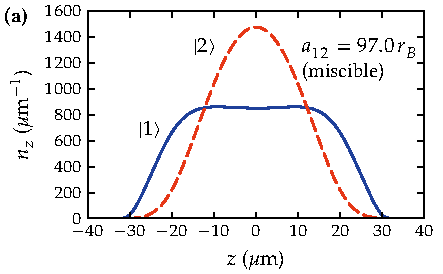
\includegraphics{figures_generated/mean_field/two_comp_gs_miscible.pdf}%
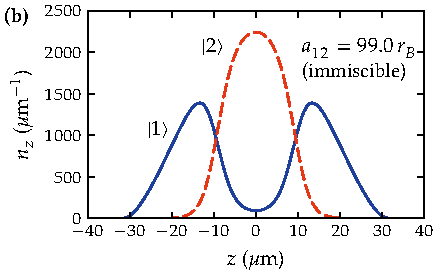
\includegraphics{figures_generated/mean_field/two_comp_gs_immiscible.pdf}}

\caption{
Two-component ground state for \textbf{(a)}~miscible and \textbf{(b)}~immiscible regimes of \Rb{} \abbrev{bec} with $N_1 = N_2 = 40,000$ atoms in a \abbrev{3d} harmonic trap with the frequencies $f_x = f_y = 97.6\un{Hz},\,f_z = 11.96\un{Hz}$.
Blue solid lines and red dashed lines show the axial density of the first and the second component respectively.
Intra-component scattering lengths are $a_{11} = 100.40\,r_B$, $a_{22} = 95.68\,r_B$, inter-component scattering length is \textbf{(a)}~$a_{12} = 97.0\,r_B$ and \textbf{(b)}~$a_{11} = 99.0\,r_B$, where $r_B$ is the Bohr radius.}%endcaption
\label{fig:bec-noise:mean-field:two-comp-gs}
\end{figure}

As an example, \figref{bec-noise:mean-field:two-comp-gs} shows the axial density $n_z = \int n(\xvec) \upd x \upd y$ of the two-component ground state for an equal mix of two states of \Rb{} \abbrev{bec}.
Two parts of the figure illustrate the difference between the miscible ($a_{12}^2 < a_{11} a_{22}$) and immiscible ($a_{12}^2 > a_{11} a_{22}$) regimes.


% =============================================================================
\subsection{Thomas-Fermi approximation}
% =============================================================================

As was mentioned earlier in this section, the starting state for the imaginary time propagation can be set to the Thomas-Fermi approximated state to minimize the propagation time.
Thomas-Fermi approximation consists of neglecting the kinetic term in the stationary equations~\eqnref{bec-noise:mean-field:cgpes-stationary}.
For a one-component state ($\Psi_2 \equiv 0$) the resulting equations can be solved analytically:
\begin{eqn}
\label{eqn:bec-noise:mean-field:tf-gs}
	| \Psi_1(\xvec) |^2 = \frac{1}{g_{11}} \max \left( \mu_1 - V_1(\xvec), 0 \right).
\end{eqn}
In the $D$-dimensional harmonic trap potential
\begin{eqn}
\label{eqn:bec-noise:mean-field:trap-potential}
	V_1(\xvec) = \frac{m}{2} \sum_{d=1}^D \omega_d^2 x_d^2
\end{eqn}
this solution has the shape of an ellipsoid with radii $r_d = \sqrt{2\mu_1 / (m \omega_d^2)}$.

The chemical potential $\mu_1$ is fixed by the normalisation condition $\int |\Psi_1|^2 \upd \xvec = N_1$.
For a \abbrev{3d} trap it can be shown to be
\begin{eqn}
	\mu_1^{\mathrm{(3D)}} =
		\left( \frac{15 N_1}{8 \pi} \right)^{\frac{2}{5}}
		\left( \frac{m \bar{\omega}^2}{2} \right)^{\frac{3}{5}}
		{g_{11}}^{\frac{2}{5}},
\end{eqn}
where $\bar{\omega} = \sqrt[3]{\omega_x \omega_y \omega_z}$.
For a \abbrev{1d} trap it has the form
\begin{eqn}
	\mu_1^{\mathrm{(1D)}} =
		\left( \frac{3 g_{11} N_1}{4} \right)^{\frac{2}{3}}
		\left( \frac{m \omega_1^2}{2} \right)^{\frac{1}{3}}.
\end{eqn}

Now we can roughly estimate the conditions necessary to drop the kinetic term from equation.
Substituting approximate solution~\eqnref{bec-noise:mean-field:tf-gs} to~\eqnref{bec-noise:mean-field:cgpes-stationary} and comparing the kinetic term with the potential term, we get the following inequation:
\begin{eqn}
\label{eqn:bec-noise:mean-field:tf-inequation}
	\frac{\hbar^2}{2m} \left(
		\frac{m \sum_{d=1}^D \omega_d^2}{2}
		+ \frac{m^2 \sum_{d=1}^D \omega_d^4 x_d^2}
			{4 \left( \mu_1 - V_1(\xvec) \right)}
	\right) \ll
	\mu \left(\mu_1 - V_1(\xvec)\right).
\end{eqn}
Near the centre of the condensate this inequation simplifies to
\begin{eqn}
\label{eqn:bec-noise:mean-field:tf-condition}
	\mu \gg \frac{\hbar}{2} |\bomega|,
\end{eqn}
where $\bomega \equiv (\omega_1, \ldots, \omega_D)^T$ is the vector of trap frequencies.

On the other hand, near the edges of the cloud the left-hand side of the inequation~\eqnref{bec-noise:mean-field:tf-inequation} diverges, while the right-hand side tends to zero.
This means that near the edges Thomas-Fermi approximation fails regardless of the conditions.
Fortunately, the density of the particles there is low, so we can estimate the width $h$ of the ``belt'' where our first approximation of the state function is significantly incorrect.
If it happens to be small as compared to the size of the condensate, the approximation can be considered valid.

The first term at the left-hand side of the inequation~\eqnref{bec-noise:mean-field:tf-inequation}
is constant and can be dropped in the limit of $V_1(\xvec) \rightarrow \mu_1$.
Then, for the sake of simplicity, we consider all but one of coordinates to be zero and the remaining one to be equal to $r_d - h_d$, where $r_d$ is the corresponding radius of the condensate.
After replacing ``$\ll$'' by ``$\approx$'' and assuming $h_d$ to be small as compared to $r_d$, we obtain the conditions for each coordinate:
\begin{eqn}
	h_d \approx \sqrt{\frac{\hbar^2}{2 \mu_1 m}},\,d \in [1, \ldots, D].
\end{eqn}
They have to be much smaller than corresponding radii, which gives us
\begin{eqn}
	\mu_1 \gg \frac{1}{2} \hbar \max_{d \in [1, \ldots, D]} \omega_d.
\end{eqn}
This conditions is less strict than the condition for the center of the condensate.
Therefore, we have only one condition justifying the application of the Thomas-Fermi approximation is~\eqnref{bec-noise:mean-field:tf-condition}.

\begin{figure}
\centerline{%
	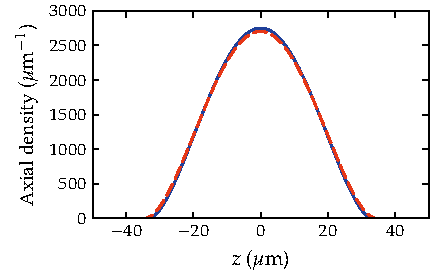
\includegraphics{figures_generated/mean_field/one_comp_gs_large.pdf}%
	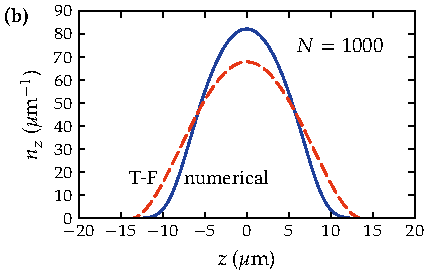
\includegraphics{figures_generated/mean_field/one_comp_gs_small.pdf}}
\caption{Numerically calculated (blue solid lines) and Thomas-Fermi approximated (red dashed lines) ground states for a one-component \Rb{} \abbrev{bec} of \textbf{(a)}~$100,000$ atoms, and \textbf{(b)}~$1,000$ atoms.}%endcaption
\label{fig:bec-noise:mean-field:tf-vs-accurate}
\end{figure}

Let us use some real-life experimental parameters and check how well the Thomas-Fermi approximation works.
For a three-dimensional trap with the frequencies $f_x = f_y = 97.6\un{Hz}$ and $f_z = 11.96\un{Hz}$ and $N_1=10^5$ \Rb{} atoms (which have the scattering length $a_{11} = 100.4 r_B$), we have $2 \mu_1 / (\hbar |\bomega|) \approx 10.68$.
This means that the Thomas-Fermi approximation produces solution which is close to the real one.
But for lower amount of atoms, say $N_1=10^3$, we get $2 \mu / (\hbar |\bomega|) \approx 1.69$, which is the sign that the we are reaching the limit of the approximation's applicability.
\figref{bec-noise:mean-field:tf-vs-accurate} shows the axial density for both cases: for $100,000$ atoms the Thomas-Fermi approximation is very close to the numerically calculated ground state, and for $1,000$ atoms it differs significantly, as expected.

More extended discussion of the Thomas-Fermi approximation can be found in~\cite{Dalfovo1999}.
It is possible to work out the Thomas-Fermi approximation for the two-component condensate, but it requires some non-trivial handling of various misibility/immiscibility cases~\cite{Anderson2010}.
